\documentclass[11pt]{article}
\usepackage{icmlko}
\begin{document}

\title{관문은 아래로 어림한다 --- 되뽑기가 학습을 63\%로 줄이기 때문에}
\author{월드모델 실험실}
\date{노트 428 · 2026년 8월 3일}
\maketitle

\begin{abstract}
노트 427이 지나가며 적은 것이 이 노트가 됐다 --- 깊이(노트 406)와
lr(노트 427) 둘 다 \textbf{실제 자료가 관문보다 좋았다}. 채택 다섯을 모아
보니 \textbf{넷에서 실제가 관문보다 크고 평균 $2.0$ 배}인데, 순위상관은
$+0.900$ 이다. \textbf{관문은 순서를 맞히고 크기를 줄여 잰다.}

기계 가설: 짝 관문은 학습 행을 \textbf{되뽑기}한다 --- $n$ 에서 $n$ 을
뽑으면 서로 다른 행이 $63.2\%$ 뿐이다. 자료가 많을수록 값이 나는 변경
(용량)은 줄어든 학습 집합에서 덜 벌 수밖에 없다. \textbf{용량이 아닌
변경(축 추가)에는 치우침이 없어야 한다} --- 대조를 같이 걸었다.

\begin{center}
\begin{tabular}{lrrrr}
\hline
변경 & 전체 & 63\% 비복원 & 되뽑기 & 전체/되뽑기 \\
\hline
\textbf{깊이 $4{\to}6$} (용량) & $\mathbf{+0.0161}$ & $+0.0089$ & $+0.0100$ & $\mathbf{1.6}$ 배 \\
\texttt{gen} 넣기 (축) & $+0.0026$ & $+0.0030$ & $+0.0027$ & $0.9$ 배 \\
\hline
\end{tabular}
\end{center}

\textbf{사전 등록 두 항이 다 맞았다.} 깊이는 전체가 제일 크고 63\% 비복원이
되뽑기와 거의 같다 --- \textbf{원인은 중복 행이 아니라 크기}다. 그리고
축 추가는 세 조건에서 평평하다.
\end{abstract}

\section{그래서 무엇을 고쳐야 하나}

관문을 버릴 일은 아니다 --- 순위상관 $+0.900$ 으로 \textbf{어느 쪽이 나은지는
맞힌다}. 틀리는 것은 \textbf{얼마나} 다. 그리고 그 틀림이 한쪽으로만 간다.

\begin{center}
\textbf{용량을 바꾸는 변경은 관문값을 \emph{아래 어림}으로 읽는다.}\\
(관문과 함께 전체 자료 차를 같이 적는다. 축·라벨·자료 추가에는 이 치우침이
없다.)
\end{center}

\section{어느 판정을 다시 봐야 하나}

용량 변경을 관문의 작은 음수로 물린 자리들이다.

\begin{center}
\begin{tabular}{lrr}
\hline
 & 관문 & 실제 \\
\hline
깊이 $6{\to}12$ (노트 412 물림) & $-0.0018$ & $-0.0012$ \\
lr $.06{\to}.10$ (노트 408 물림) & $+0.0005$ & $+0.0028$ \\
\hline
\end{tabular}
\end{center}

\textbf{둘 다 이미 다시 봤고 둘 다 채택됐다}(노트 426 · 427) --- 다만 그때는
\emph{전이}가 근거였다. 이 노트는 \textbf{판만 보고도 다시 봤어야 했다}는
것을 말한다. 남은 것은 \textbf{$K$} 다 --- 노트 396이 ``$K{=}64$ 는
포화''라 적었는데 그것도 용량이고 관문으로 잰 것이다.

\section{한계}

변경 \textbf{둘}로 잰 치우침이다. 용량 쪽이 하나(깊이), 대조가 하나(gen).
``용량이면 $1.6$ 배''라고 상수를 쓸 근거는 없다 --- 이 노트가 주장하는 것은
\textbf{부호와 방향}이지 계수가 아니다. 그리고 $63.2\%$ 는 되뽑기의 산술이지
관문이 그 크기를 고른 것이 아니다.

\begin{tabular}{lp{7.0cm}}
\hline
$K{=}64$ & 관문으로 물린 마지막 용량 손잡이. 아래 어림이었다면 살아 있다 \\
관문을 바꿀까 & 유보 행을 되뽑으면 학습이 온전하다. 다만 그것은 \emph{다른}
불확실성(유보 표본)을 재는 것이라 바꾸면 옛 수치와 못 견준다 \\
치우침의 크기 & 변경 여럿으로 다시 재야 계수를 말할 수 있다 \\
\hline
\end{tabular}

\begin{figure}[h]
\centering
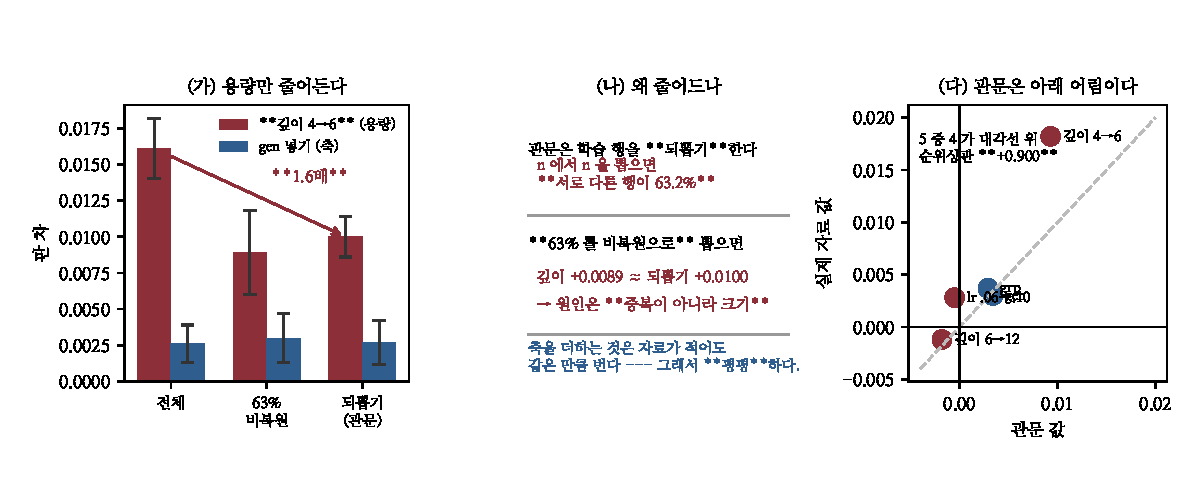
\includegraphics[width=\textwidth]{figs/fig428.pdf}
\caption{(가) 용량 변경만 줄어든다. (나) 원인은 크기다 --- 63\% 비복원이
되뽑기와 같다. (다) 채택 다섯 중 넷이 대각선 위.}
\end{figure}

\end{document}
